\documentclass[]{article}
\usepackage{graphicx}
\usepackage{amsmath}
\usepackage[a4paper,bindingoffset=0.2in,%
left=1.2in,right=1.2in,top=1.2in,bottom=1.2in,%
footskip=.25in]{geometry}
\usepackage{caption}
\usepackage{subcaption}

%opening
\title{A Note on GMM Estimation of Theories of Expectation Formation}
\author{Tao Wang}

\begin{document}

\maketitle

\section{A Generic Framework}

For a given process of inflation and a particular theory of expectation formation, the GMM estimate of the vector of parameters $\Omega$ is defined as the following. 

\begin{eqnarray}
\widehat \Omega = \underset{\Omega }{argmin} (M_{\textrm{data} } - F(\Omega, Y)) W  (M_{\textrm{data} } - F(\Omega, Y))'
\end{eqnarray}

\begin{itemize}
	\item  $\Omega$ is a vector of size of $k$, depending on the number of parameters to be estimated. 
	\item $M_{data}$ is the moments computed from data, i.e. mean forecasts, average forecast errors, the average cross-sectional variance of forecasts (disagreement), average uncertainty, etc. Also the autocovariance of all the abovementioned.  
	
	\item $F$ is the moments that are generated from a certain theory of expectation formation and inflation process. It is a function of parameters $\Omega$ as well as the $Y$, the real-time data(including history) that is available to forecasters at each point of the time $t$. 
	\item For instance, for $T$ periods, $Y$ includes $T$  sequences of real-time inflation data of different lengths that terminate at each point of the forecasting:  $t =0$, $t=1$... $t=T$ . 
	\item  Both $M$ and $F$ is of the size  $m$, depending on the number of moments used for estimation. For instance, if we only estimate expectation formation using mean forecasts, disagreements and forecast errors while taking the inflation process as given, there are three moments, thus $m = 3$. If we include autocovariance of forecast errors, then $m=4$.  
	
	\item $W$ is the weighting matrix. For now, I stick to the identity matrix. 
\end{itemize}

The above procedure is specific to a pair of an assumed inflation process and a theory of expectation. It can be estimated only estimated for the theory of expectation formation with exogenous fed parameters of the inflation process using the entire history of inflation data, or we could jointly estimate the parameters of expectation formation and the inflation process. 

\section{Estimation}
\subsection{Real-time Data}

When agents form their expectations of inflation at any point of the time, what is potentially available to them is the real-time inflation data, namely those released from the most update-to-date vintage of the inflation. In order to match as close as possible the information set available to the forecasting agents, we need to use real-time data for each particular point of time.  

These real-time vintage inflation data since 1998 were obtained from the Real-Time Data Research Center hosted by the Federal Reserve Bank of Philadelphia. 

To get an idea of how much of the differences there are between the real-time inflation and the most recent vintage in 2018, Figure \ref{real_time_rev} and \ref{ts_real_time_current_vintage} plot, respectively, the distributions of the revisions as well as the time series of the inflation. Although overall, there is no obvious skewness of the revisions, there have been indeed sizable revisions made for the real-time data. 

\begin{figure}[ht]
		\centering
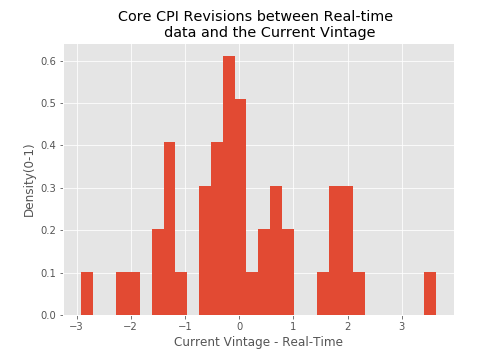
\includegraphics[width=0.7\textwidth]{figures/hist_rev_realtime.png}
\caption{Revisions of Current-vintage from Real-time Core CPI}
\label{real_time_rev}
	\begin{flushleft}
	{\footnotesize Note: real-time data  at time $t$ is defined the inflation from $t-1$ to $t$ according to the most recent vintage of CPI inflation at time $t$. The period is between 2000 M1-2018 M3.}
\end{flushleft}
\end{figure}


\begin{figure}[ht]
	\centering
	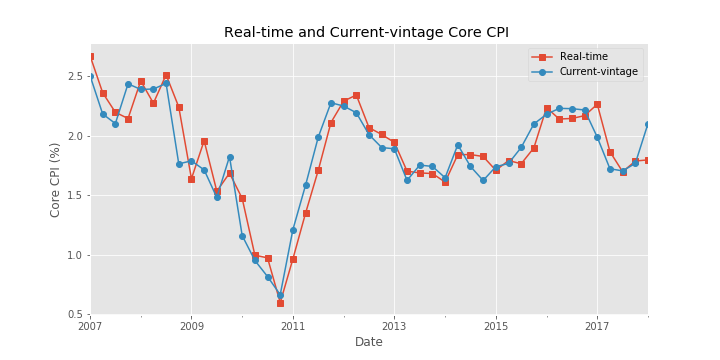
\includegraphics[width=0.8\textwidth]{figures/ts_rev_realtime.png}
	\caption{Current-vintage and Real-time Core CPI}
	\label{ts_real_time_current_vintage}
\end{figure}

\subsection{Results}

\subsubsection{Professional Forecasters}

Figure \ref{SE_diag_SPF} and \ref{SE_diag_joint_SPF} plot the estimated moments for SE model together with the data moments professional forecasts of SPF. 

From left to the right, the four columns of the figures are based on estimation 

\begin{figure}[ht]
	\centering
	\begin{subfigure}[b]{\textwidth}
		\centering
		\caption{Estimation of SE}
		\label{SE_diag_SPF}
		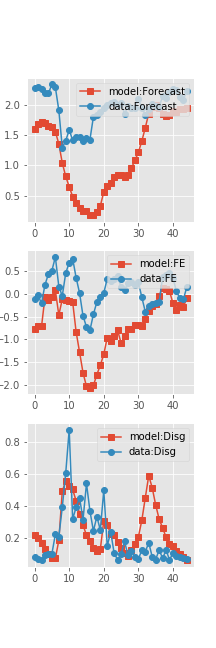
\includegraphics[width=0.24\textwidth]{figures/spf_se_est_diag0.png}
		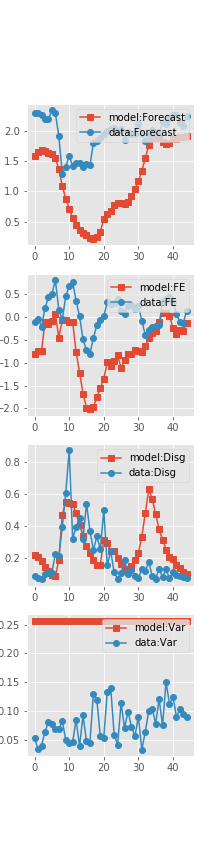
\includegraphics[width=0.24\textwidth]{figures/spf_se_est_diag1.png}
		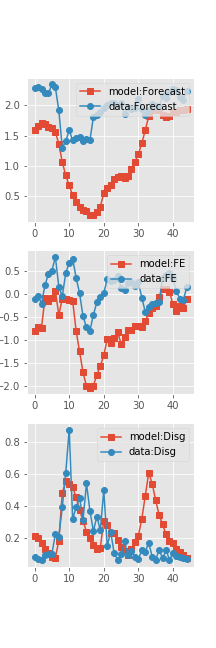
\includegraphics[width=0.24\textwidth]{figures/spf_se_est_diag2.png}
		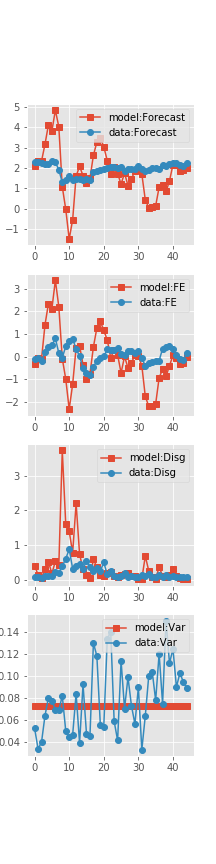
\includegraphics[width=0.24\textwidth]{figures/spf_se_est_diag3.png}
	\end{subfigure}
	\vspace{1em}
	\vfill
	\begin{subfigure}[b]{\textwidth}
		\centering
		\caption{Joint Estimation of SE and Inflation Process}
		\label{SE_diag_joint_SPF}
	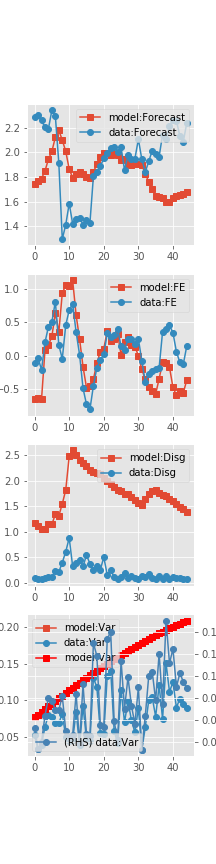
\includegraphics[width=0.24\textwidth]{figures/spf_se_est_joint_diag0.png}
	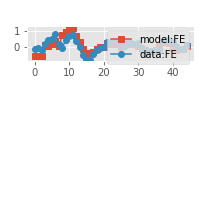
\includegraphics[width=0.24\textwidth]{figures/spf_se_est_joint_diag1.png}
	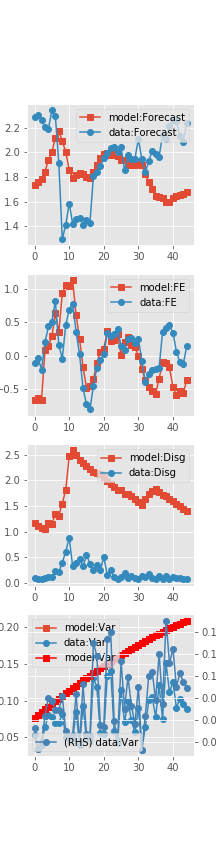
\includegraphics[width=0.24\textwidth]{figures/spf_se_est_joint_diag2.png}
	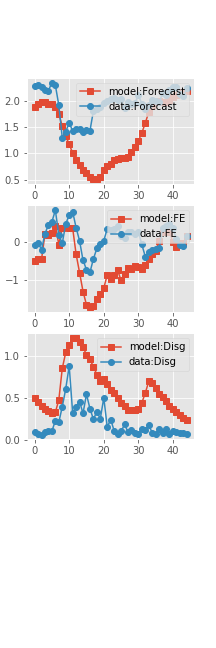
\includegraphics[width=0.24\textwidth]{figures/spf_se_est_joint_diag3.png}
	\end{subfigure}
	\\
	\begin{flushleft}
		{\footnotesize Note: the upper panel estimates expectation formation only taking the process of inflation parameters as given. The bottom panel estimates the parameters of expectation formation and inflation process jointly. From left to the right, the moments used are $\overline y_{t|t}$, $\overline{FE}_{t}$, $\overline y_{t|t}$/$\overline{FE}_{t}$ and $\overline y_{t|t}$ / $\overline{FE}_{t}$/ $\overline{\textrm{Disg}_t}$, respectively. }
	\end{flushleft}
	\caption{SE of Professionals: Esimated Model Moments and Data Moments}
\end{figure}


\begin{figure}[ht]
	\centering
	\begin{subfigure}[b]{\textwidth}
		\centering
		\caption{Estimation of NI}
		\label{NI_diag_SPF}
		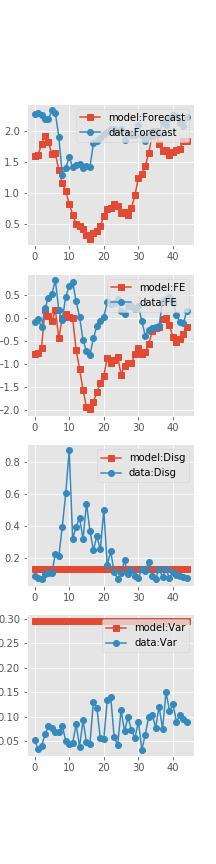
\includegraphics[width=0.24\textwidth]{figures/spf_ni_est_diag0.png}
		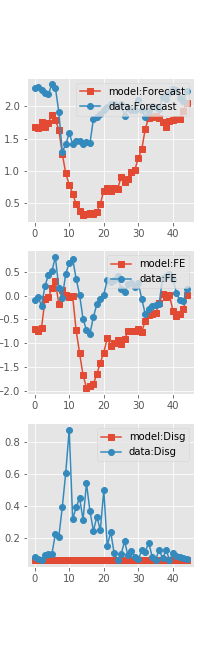
\includegraphics[width=0.24\textwidth]{figures/spf_ni_est_diag1.png}
		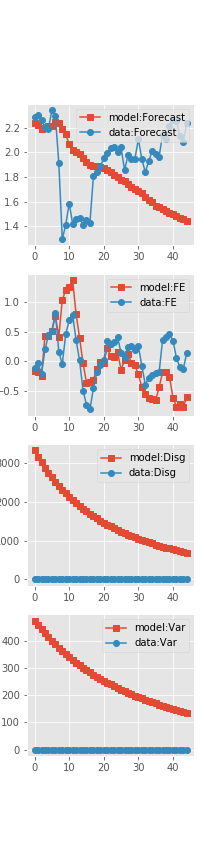
\includegraphics[width=0.24\textwidth]{figures/spf_ni_est_diag2.png}
		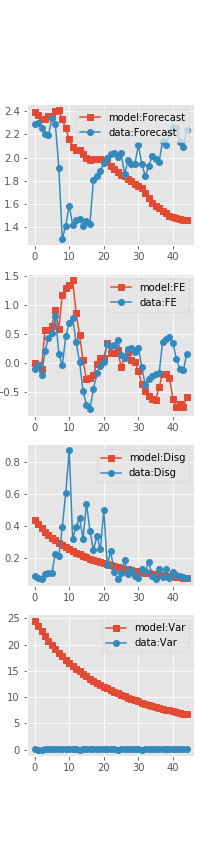
\includegraphics[width=0.24\textwidth]{figures/spf_ni_est_diag3.png}
	\end{subfigure}
	\vspace{1em}
	\vfill
	\begin{subfigure}[b]{\textwidth}
		\centering
		\caption{Joint Estimation of NI and Inflation Process}
		\label{NI_diag_joint_SPF}
		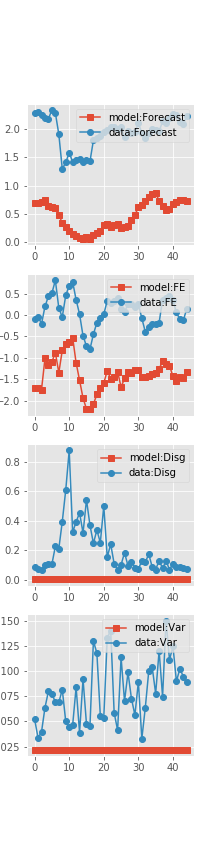
\includegraphics[width=0.24\textwidth]{figures/spf_ni_est_joint_diag0.png}
		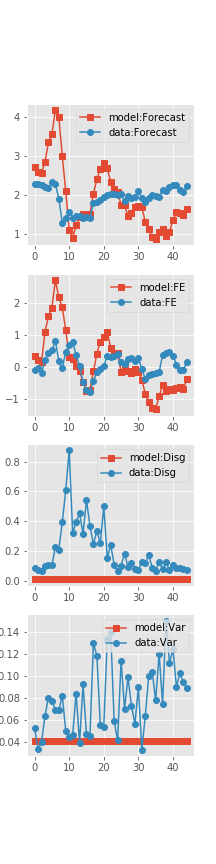
\includegraphics[width=0.24\textwidth]{figures/spf_ni_est_joint_diag1.png}
		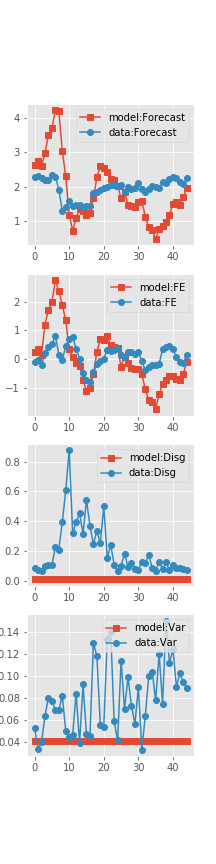
\includegraphics[width=0.24\textwidth]{figures/spf_ni_est_joint_diag2.png}
		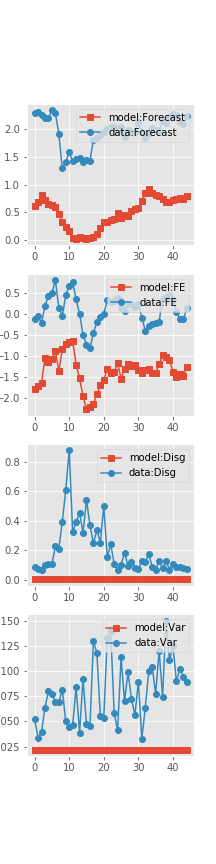
\includegraphics[width=0.24\textwidth]{figures/spf_ni_est_joint_diag3.png}
	\end{subfigure}
	\\
	\begin{flushleft}
		{\footnotesize Note: the upper panel estimates expectation formation only taking the process of inflation parameters as given. The bottom panel estimates the parameters of expectation formation and inflation process jointly. From left to the right, the moments used are $\overline y_{t|t}$, $\overline{FE}_{t}$, $\overline y_{t|t}$/$\overline{FE}_{t}$ and $\overline y_{t|t}$ / $\overline{FE}_{t}$/ $\overline{\textrm{Disg}_t}$, respectively. }
	\end{flushleft}
	\caption{NI of Professionals: Esimated Model Moments and Data Moments}
\end{figure}

\subsubsection{Households}

\begin{figure}[ht]
	\centering
	\begin{subfigure}[b]{\textwidth}
		\centering
		\caption{Estimation of SE}
		\label{SE_diag_SCE}
		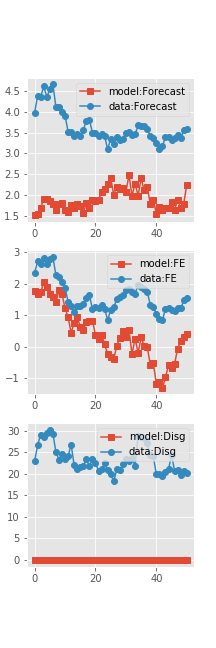
\includegraphics[width=0.24\textwidth]{figures/sce_se_est_diag0.png}
		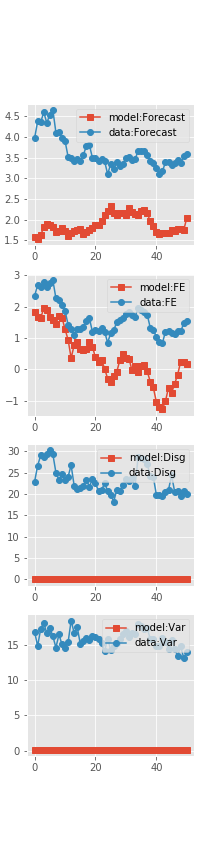
\includegraphics[width=0.24\textwidth]{figures/sce_se_est_diag1.png}
		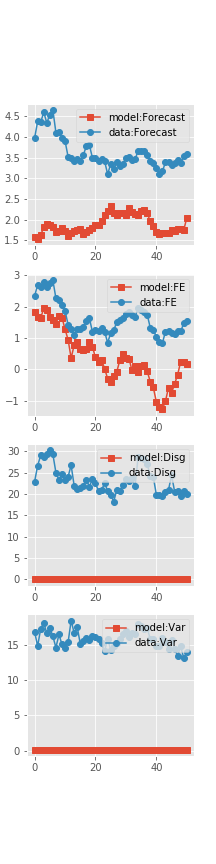
\includegraphics[width=0.24\textwidth]{figures/sce_se_est_diag2.png}
		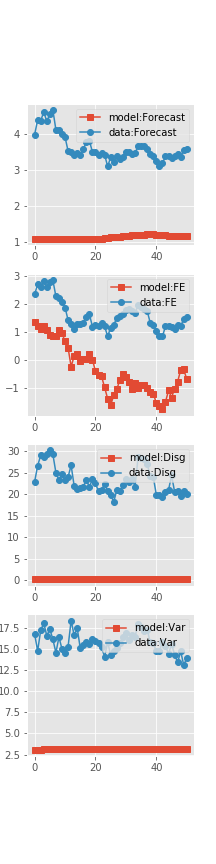
\includegraphics[width=0.24\textwidth]{figures/sce_se_est_diag3.png}
	\end{subfigure}
	\vspace{1em}
	\vfill
	\begin{subfigure}[b]{\textwidth}
		\centering
		\caption{Joint Estimation of SE and Inflation Process}
		\label{SE_diag_joint_SCE}
		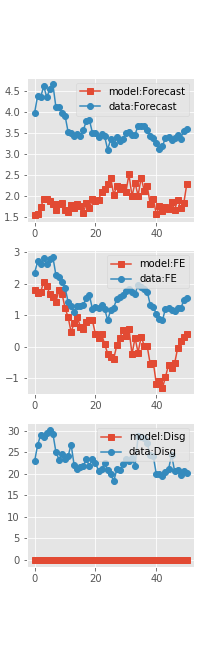
\includegraphics[width=0.24\textwidth]{figures/sce_se_est_joint_diag0.png}
		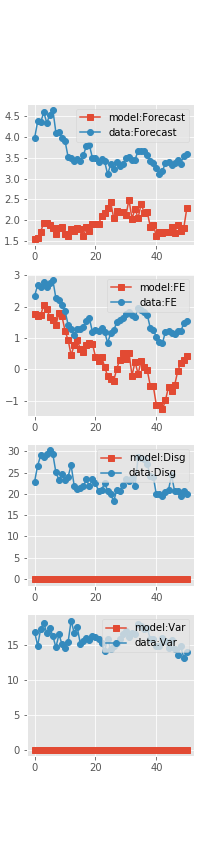
\includegraphics[width=0.24\textwidth]{figures/sce_se_est_joint_diag1.png}
		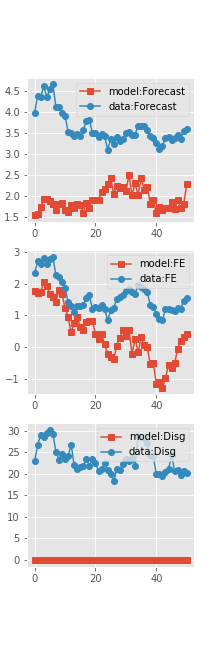
\includegraphics[width=0.24\textwidth]{figures/sce_se_est_joint_diag2.png}
		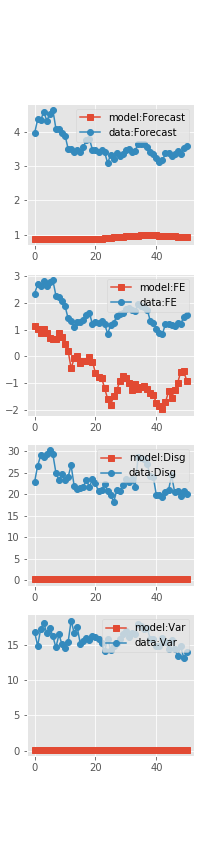
\includegraphics[width=0.24\textwidth]{figures/sce_se_est_joint_diag3.png}
	\end{subfigure}
	\\
	\begin{flushleft}
		{\footnotesize Note: the upper panel estimates expectation formation only taking the process of inflation parameters as given. The bottom panel estimates the parameters of expectation formation and inflation process jointly. From left to the right, the moments used are $\overline y_{t|t}$, $\overline{FE}_{t}$, $\overline y_{t|t}$/$\overline{FE}_{t}$ and $\overline y_{t|t}$ / $\overline{FE}_{t}$/ $\overline{\textrm{Disg}_t}$, respectively.}
	\end{flushleft}
	\caption{SE of Households: Esimated Model Moments and Data Moments}
\end{figure}


\begin{figure}[ht]
	\centering
	\begin{subfigure}[b]{\textwidth}
		\centering
		\caption{Estimation of NI}
		\label{NI_diag_SCE}
		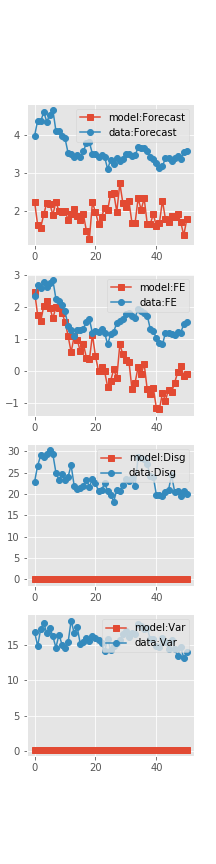
\includegraphics[width=0.24\textwidth]{figures/sce_ni_est_diag0.png}
		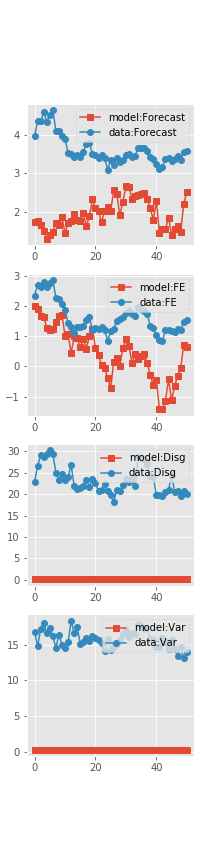
\includegraphics[width=0.24\textwidth]{figures/sce_ni_est_diag1.png}
		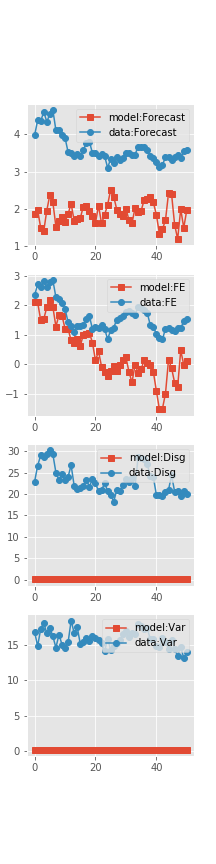
\includegraphics[width=0.24\textwidth]{figures/sce_ni_est_diag2.png}
		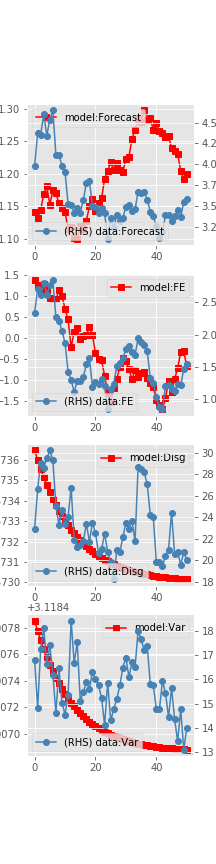
\includegraphics[width=0.24\textwidth]{figures/sce_ni_est_diag3.png}
	\end{subfigure}
	\vspace{1em}
	\vfill
	\begin{subfigure}[b]{\textwidth}
		\centering
		\caption{Joint Estimation of SE and Inflation Process}
		\label{NI_diag_joint_SCE}
		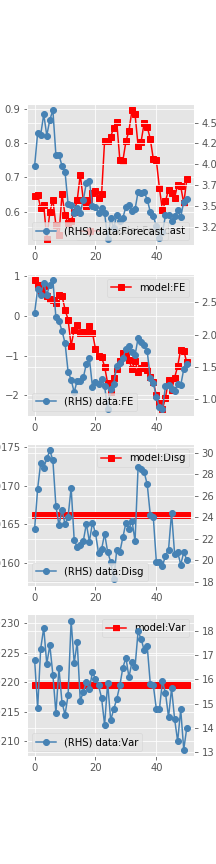
\includegraphics[width=0.24\textwidth]{figures/sce_ni_est_joint_diag0.png}
		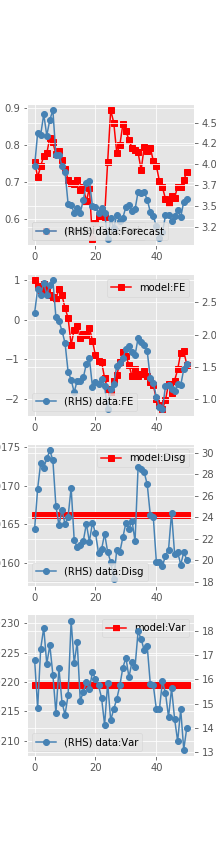
\includegraphics[width=0.24\textwidth]{figures/sce_ni_est_joint_diag1.png}
		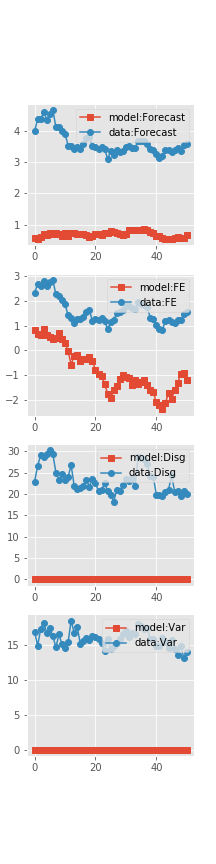
\includegraphics[width=0.24\textwidth]{figures/sce_ni_est_joint_diag2.png}
		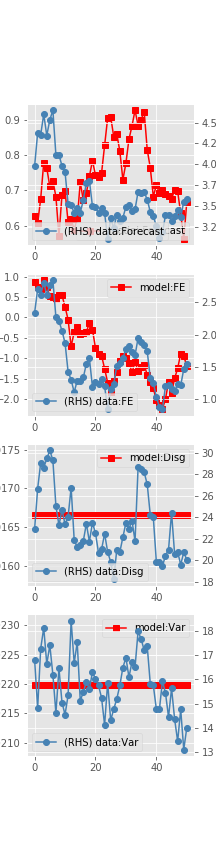
\includegraphics[width=0.24\textwidth]{figures/sce_ni_est_joint_diag3.png}
	\end{subfigure}
	\\
	\begin{flushleft}
		{\footnotesize Note: the upper panel estimates expectation formation only taking the process of inflation parameters as given. The bottom panel estimates the parameters of expectation formation and inflation process jointly. From left to the right, the moments used are $\overline y_{t|t}$, $\overline{FE}_{t}$, $\overline y_{t|t}$/$\overline{FE}_{t}$ and $\overline y_{t|t}$ / $\overline{FE}_{t}$/ $\overline{\textrm{Disg}_t}$, respectively. }
	\end{flushleft}
	\caption{NI of Households: Esimated Model Moments and Data Moments}
\end{figure}



\end{document}
